% !TeX root = ../main.tex

\section{Progettazione Concettuale}
In questa fase si individuano e si modellano i concetti rilevanti del dominio applicativo, indipendentemente dagli aspetti implementativi o tecnologici. L'obiettivo è costruire uno schema \textbf{Entità-Relazione} che descriva in modo chiaro le entità del sistema, i loro attributi, le associazioni tra esse e i vincoli principali imposti dalla traccia.

La progettazione è stata sviluppata in due momenti distinti: una prima modellazione completa del dominio mediante uno schema ER esteso, e una successiva ristrutturazione del modello, finalizzata a semplificarne la struttura senza alterarne il contenuto informativo essenziale.

\subsection{Schema Entità-Relazioni (ER)}
\begin{figure}[H]
  \begin{center}
    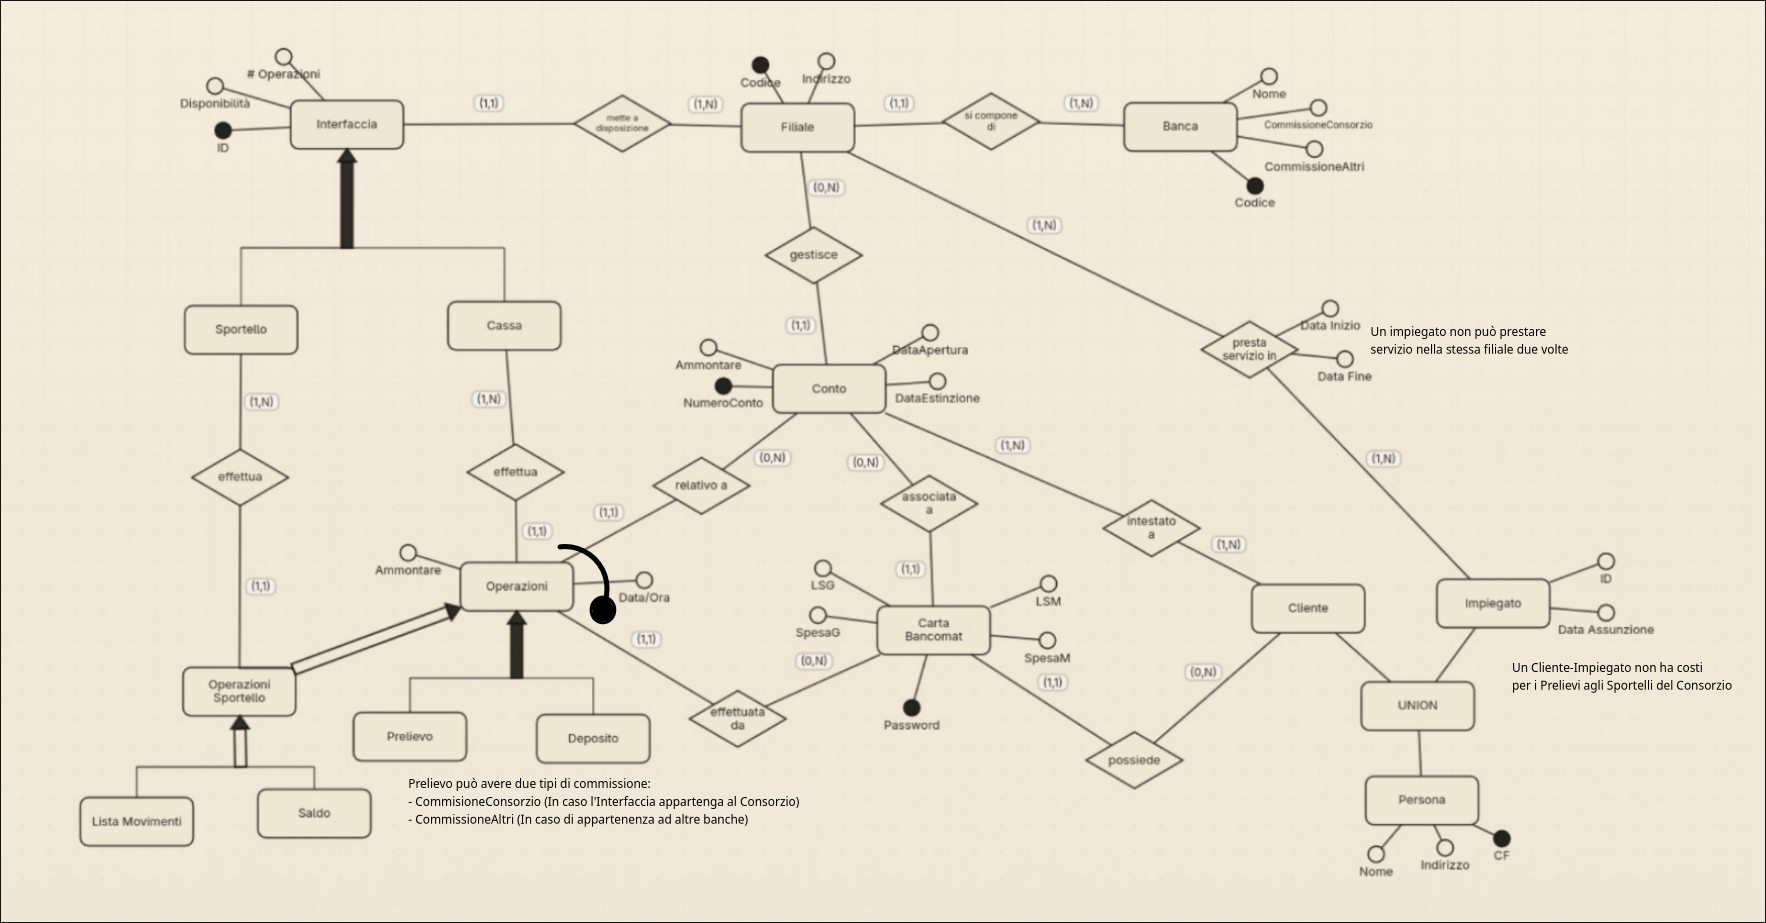
\includegraphics[width=0.95\textwidth]{../imgs/modelloER.png}
  \end{center}
  \caption{Schema Entità-Relazione iniziale del Consorzio Bancario}
  \label{fig:er_model}
\end{figure}

\subsection{Analisi dello schema}
Lo schema concettuale descrive una rete bancaria informatizzata costituita da più banche appartenenti a un medesimo consorzio e dotate di filiali, impiegati, conti, carte Bancomat e postazioni operative per l'esecuzione delle operazioni bancarie.

Nel modello iniziale si è scelto di rappresentare in modo esplicito alcune differenze semantiche attraverso gerarchie di specializzazione, in particolare per distinguere i diversi tipi di interfaccia e i diversi tipi di operazione.

\subsubsection{Entità e gerarchie}

\begin{itemize}
  \item \textbf{Banca}: ente bancario appartenente al consorzio, identificato da un codice e dotato di un nome. Per ciascuna banca vengono inoltre memorizzate le commissioni applicate ai prelievi effettuati presso sportelli del consorzio o presso sportelli di altre banche.\\
  Attributi: \textit{Codice} (chiave primaria), \textit{Nome}, \textit{CommissioneConsorzio}, \textit{CommissioneAltri}.

  \item \textbf{Filiale}: sede operativa di una banca. Ogni filiale è caratterizzata da un proprio codice e da un indirizzo; presso di essa vengono gestiti i conti, lavorano gli impiegati e sono messe a disposizione le interfacce operative.\\
  Attributi: \textit{Codice} (chiave primaria), \textit{Indirizzo}.

  \item \textbf{Persona}: entità generale che raccoglie le informazioni anagrafiche comuni ai soggetti del sistema.\\
  Attributi: \textit{CF} (chiave primaria), \textit{Nome}, \textit{Indirizzo}.

  \item \textbf{Cliente}: entità che rappresenta i soggetti intestatari di conti e possessori di carte Bancomat.\\
  Attributi: ereditati da \textbf{Persona}.

  \item \textbf{Impiegato}: entità che rappresenta i dipendenti della banca.\\
  Attributi: \textit{ID}, \textit{Data Assunzione}, oltre agli attributi comuni ereditati da \textbf{Persona}.

  \item \textbf{Conto}: rapporto bancario relativo a uno o più clienti e gestito da una filiale.\\
  Attributi: \textit{Numero Conto} (chiave primaria), \textit{Data Apertura}, \textit{Data Estinzione}, \textit{Ammontare}.

  \item \textbf{Carta Bancomat}: strumento associato a un conto e utilizzabile per l'esecuzione delle operazioni bancarie.\\
  Attributi: \textit{Password} (chiave primaria), \textit{Limite Spesa Giornaliero(LSG)}, \textit{Limite Spesa Mensile(LSM)}, \textit{SpesaG}, \textit{SpesaM}.

  \item \textbf{Interfaccia}: postazione operativa presso cui possono essere eseguite operazioni bancarie.\\
  Attributi: \textit{ID} (chiave primaria), \textit{Disponibilità}, \textit{\#Operazioni}.

  \item \textbf{Cassa}: specializzazione di \textbf{Interfaccia}. Rappresenta una postazione di cassa fisica presente presso una filiale.\\
  Attributi: ereditati da \textbf{Interfaccia}.

  \item \textbf{Sportello}: specializzazione di \textbf{Interfaccia}. Rappresenta uno sportello automatico.\\
  Attributi: ereditati da \textbf{Interfaccia}.

  \item \textbf{Operazioni}: entità che rappresenta una generica operazione bancaria eseguita su un conto.\\
  Attributi: \textit{Data/Ora}, \textit{Ammontare}.

  \item \textbf{Prelievo}: specializzazione di \textbf{Operazioni}.\\
  Attributi: ereditati da \textbf{Operazioni}.

  \item \textbf{Deposito}: specializzazione di \textbf{Operazioni}.\\
  Attributi: ereditati da \textbf{Operazioni}.

  \item \textbf{Operazioni Sportello}: specializzazione di \textbf{Operazioni} che raccoglie le operazioni specificamente modellate per lo sportello automatico.\\
  Attributi: ereditati da \textbf{Operazioni}.

  \item \textbf{Saldo}: specializzazione di \textbf{Operazioni Sportello}.\\
  Attributi: ereditati da \textbf{Operazioni Sportello}.

  \item \textbf{Lista Movimenti}: specializzazione di \textbf{Operazioni Sportello}.\\
  Attributi: ereditati da \textbf{Operazioni Sportello}.
\end{itemize}

Nel modello iniziale:
\begin{itemize}
  \item \textbf{Interfaccia} è specializzata in \textbf{Cassa} e \textbf{Sportello} mediante una gerarchia \textbf{totale e disgiunta};
  \item \textbf{Operazioni} è specializzata in \textbf{Prelievo}, \textbf{Deposito} e \textbf{Operazioni Sportello} mediante una gerarchia \textbf{totale e disgiunta};
  \item \textbf{Operazioni Sportello} è ulteriormente specializzata in \textbf{Saldo} e \textbf{Lista Movimenti} mediante una gerarchia \textbf{parziale e disgiunta};
  \item \textbf{Persona} raccoglie gli attributi comuni a \textbf{Cliente} e \textbf{Impiegato}, consentendo di rappresentare il caso in cui uno stesso soggetto possa appartenere a entrambi i ruoli.
\end{itemize}

\subsubsection{Relazioni}

\begin{itemize}
  \item \textbf{Si compone di} (\textbf{Banca} $\rightleftarrows$ \textbf{Filiale}): rappresenta l'appartenenza di una filiale a una banca.\\
  Cardinalità:
  \begin{itemize}
    \item una banca si compone di una o più filiali \((1,N)\);
    \item una filiale appartiene a una sola banca \((1,1)\).
  \end{itemize}

  \item \textbf{Mette a disposizione} (\textbf{Filiale} $\rightleftarrows$ \textbf{Interfaccia}): associa a ciascuna filiale le interfacce operative presenti presso di essa.\\
  Cardinalità:
  \begin{itemize}
    \item una filiale mette a disposizione una o più interfacce \((1,N)\);
    \item un'interfaccia appartiene a una sola filiale \((1,1)\).
  \end{itemize}

  \item \textbf{Gestisce} (\textbf{Filiale} $\rightleftarrows$ \textbf{Conto}): collega ciascun conto alla filiale che lo gestisce.\\
  Cardinalità:
  \begin{itemize}
    \item una filiale può gestire zero o più conti \((0,N)\);
    \item un conto è gestito da una sola filiale \((1,1)\).
  \end{itemize}

  \item \textbf{Intestata a} (\textbf{Conto} $\rightleftarrows$ \textbf{Cliente}): rappresenta l'intestazione del conto a uno o più clienti.\\
  Cardinalità:
  \begin{itemize}
    \item un conto è intestato a uno o più clienti \((1,N)\);
    \item un cliente può essere intestatario di uno o più conti \((1,N)\).
  \end{itemize}

  \item \textbf{Associata a} (\textbf{Carta Bancomat} $\rightleftarrows$ \textbf{Conto}): collega ogni carta al conto cui essa è riferita.\\
  Cardinalità:
  \begin{itemize}
    \item una carta Bancomat è associata a un solo conto \((1,1)\);
    \item un conto può avere zero o più carte associate \((0,N)\).
  \end{itemize}

  \item \textbf{Possiede} (\textbf{Cliente} $\rightleftarrows$ \textbf{Carta Bancomat}): rappresenta il possesso della carta da parte del cliente.\\
  Cardinalità:
  \begin{itemize}
    \item un cliente può possedere zero o più carte Bancomat \((0,N)\);
    \item una carta Bancomat è posseduta da un solo cliente \((1,1)\).
  \end{itemize}

  \item \textbf{Relativo a} (\textbf{Operazioni} $\rightleftarrows$ \textbf{Conto}): collega ogni operazione al conto cui essa si riferisce.\\
  Cardinalità:
  \begin{itemize}
    \item un conto può essere coinvolto in zero o più operazioni \((0,N)\);
    \item ogni operazione è relativa a un solo conto \((1,1)\).
  \end{itemize}

  \item \textbf{Effettuata da} (\textbf{Operazioni} $\rightleftarrows$ \textbf{Carta Bancomat}): collega una operazione alla carta utilizzata.\\
  Cardinalità:
  \begin{itemize}
    \item un'operazione deve essere effettuata da una sola carta Bancomat \((1,1)\);
    \item una carta Bancomat può essere utilizzata per zero o più operazioni \((0,N)\).
  \end{itemize}

  \item \textbf{Effettua} (\textbf{Cassa} $\rightleftarrows$ \textbf{Operazioni}): indica le operazioni eseguite tramite una cassa.\\
  Cardinalità:
  \begin{itemize}
    \item una cassa può effettuare una o più operazioni \((1,N)\);
    \item ogni operazione è eseguita da una sola cassa \((1,1)\).
  \end{itemize}

  \item \textbf{Effettua} (\textbf{Sportello} $\rightleftarrows$ \textbf{Operazioni Sportello}): indica le operazioni eseguite tramite sportello automatico.\\
  Cardinalità:
  \begin{itemize}
    \item uno sportello può effettuare una o più operazioni \((1,N)\);
    \item ogni operazione di sportello è eseguita da un solo sportello \((1,1)\).
  \end{itemize}

  \item \textbf{Presta servizio in} (\textbf{Impiegato} $\rightleftarrows$ \textbf{Filiale}): rappresenta l'assegnazione dell'impiegato a una filiale.\\
  Cardinalità:
  \begin{itemize}
    \item una filiale impiega uno o più impiegati \((1,N)\);
    \item ciascun impiegato presta servizio in una filiale \((1,N)\).
  \end{itemize}
  Attributi della relazione:
  \begin{itemize}
    \item \textit{DataInizio}: data di inizio del servizio presso la filiale;
    \item \textit{DataFine}: data di termine del servizio presso la filiale.
  \end{itemize}
\end{itemize}

\subsubsection{Attributi derivati e osservazioni}

Nel modello iniziale l'attributo \textit{\#Operazioni} di \textbf{Interfaccia} è da considerarsi \textbf{derivato}, in quanto ricavabile dal conteggio delle operazioni eseguite dalla singola interfaccia.

Anche gli attributi \textit{SpesaG} e \textit{SpesaM} associati alla \textbf{Carta Bancomat} possono essere interpretati come valori mantenuti e aggiornati sulla base delle operazioni registrate in determinati intervalli temporali.

\subsection{Vincoli}
Alcuni vincoli richiesti dalla traccia non sono esprimibili in modo completo mediante il solo formalismo grafico ER e devono quindi essere specificati testualmente.

\begin{itemize}
  \item Un impiegato può prestare servizio solo presso filiali appartenenti alla propria banca.
  \item Un impiegato deve permanere in una filiale per almeno un mese prima di poter essere trasferito.
  \item Un cliente può essere anche impiegato della stessa banca.
  \item Un conto estinto deve avere \textit{Ammontare} nullo oppure pari a zero.
  \item L'importo di un prelievo non può essere superiore alla disponibilità dell'interfaccia presso cui viene effettuato.
  \item L'importo di un prelievo non può superare il limite di spesa giornaliero o mensile della carta Bancomat utilizzata.
  \item Le commissioni associate ai prelievi dipendono dal fatto che lo sportello appartenga a una banca del consorzio oppure a una banca esterna.
  \item Un cliente che sia anche impiegato della stessa banca non sostiene costi di gestione per le operazioni effettuate presso filiali della banca stessa o presso sportelli del consorzio.
\end{itemize}

\subsection{Analisi dei cicli}
Nel modello sono presenti percorsi multipli tra alcune entità, in particolare tra \textbf{Cliente}, \textbf{Conto}, \textbf{Carta Bancomat} e \textbf{Operazioni}. Questi tuttavia, non introducono ambiguità concettuali, poiché ciascuna relazione esprime un significato distinto: l'intestazione del conto, il possesso della carta, l'associazione tra carta e conto e l'esecuzione delle operazioni.

Si può quindi concludere che \textbf{non} emergono cicli problematici dal punto di vista concettuale; le eventuali dipendenze sono controllate tramite cardinalità e vincoli applicativi.
